The energy deposit measured per event by CASTOR can be shown as a 2D histogram with 16x14 pixels. The information of the amount of energy deposit is transmitted through the intensity of the colour. With a convolutional neural network it should be possible to learn the distinctive patterns of different types of particles and therefore to classify events correctly. 

\section{Data}
To train the network a sufficiently high amount of simulations are needed. For training and validation Monte Carlo events generated by the PYTHIA8 and the EPOS generator are used. To separate actual events from background noise a typical minimum bias event selection was made. Only events which trigger an energetic response higher than 5 GeV in the CaloTowers with a pseudorapidity range of 3.1 < $|\eta|$ < 5 are used in the analysis. To simplify the work for the neural network, only events containing isolated particles in CASTOR are used for differentiation. Here an isolated particle is defined by a minimum distance of $\Delta$R = $\sqrt{(\Delta \phi)^2 + (\Delta \eta)^2}$ = 0.8 to the next particles generated by the same event. Therefore every generated event is checked for isolated particles travelling through CASTOR.

Within CASTOR different types of particles leave different characteristic signatures which can be used to identify the particles. In fig. \ref{signals} the different types of signals can be seen. Electromagnetic light particles, such as electrons, positrons and photons, have a very large cross section and interact with the electromagnetic part of the calorimeter. In the energy deposit histogram very high energies are measured within the first two sections while nearly no energy is deposited in the hadronic rear sections.
When hadrons reach the calorimeter they interact and produce several lighter secondary particles which in turn interact again. The energy deposit is therefore distributed wider and reaches its peak within the hadronic sections of the calorimeter.
Muons very sparsely interact with the material of the calorimeter and pass it nearly without losing energy. A muon track is normally contained within one tower but can be seen as a very small energy deposit in every section.

Every histogram containing the energy deposit has a corresponding label vector. This is a binary vector, where the first index corresponds to isolated electron, positron or photon, the second to isolated hadron and the third to background. Here background is everything besides an isolated electron/photon or hadron. Therefore the categories do not exclude each other, since it is possible that an isolated electron and an isolated hadron travel through CASTOR in the same event. In table \ref{particlecounts} the particles and their frequency are listed. For this 500.000 Monte Carlo events are evaluated and only those particles with the beforementioned minimum distance are counted. For a neural network typically at least 1000 samples per class are needed to pick up the identifying features. As can be seen most particles are too few for a full training, whereas the differentiation between electrons/photons (which produce nearly the same signal) and hadrons seems possible. Even though muons have an especially distinctive signal, their number is too small to include them as a separate category.

\begin{figure}
\centering
\begin{minipage}[t]{0.95\textwidth}
\begin{minipage}{0.45\textwidth}
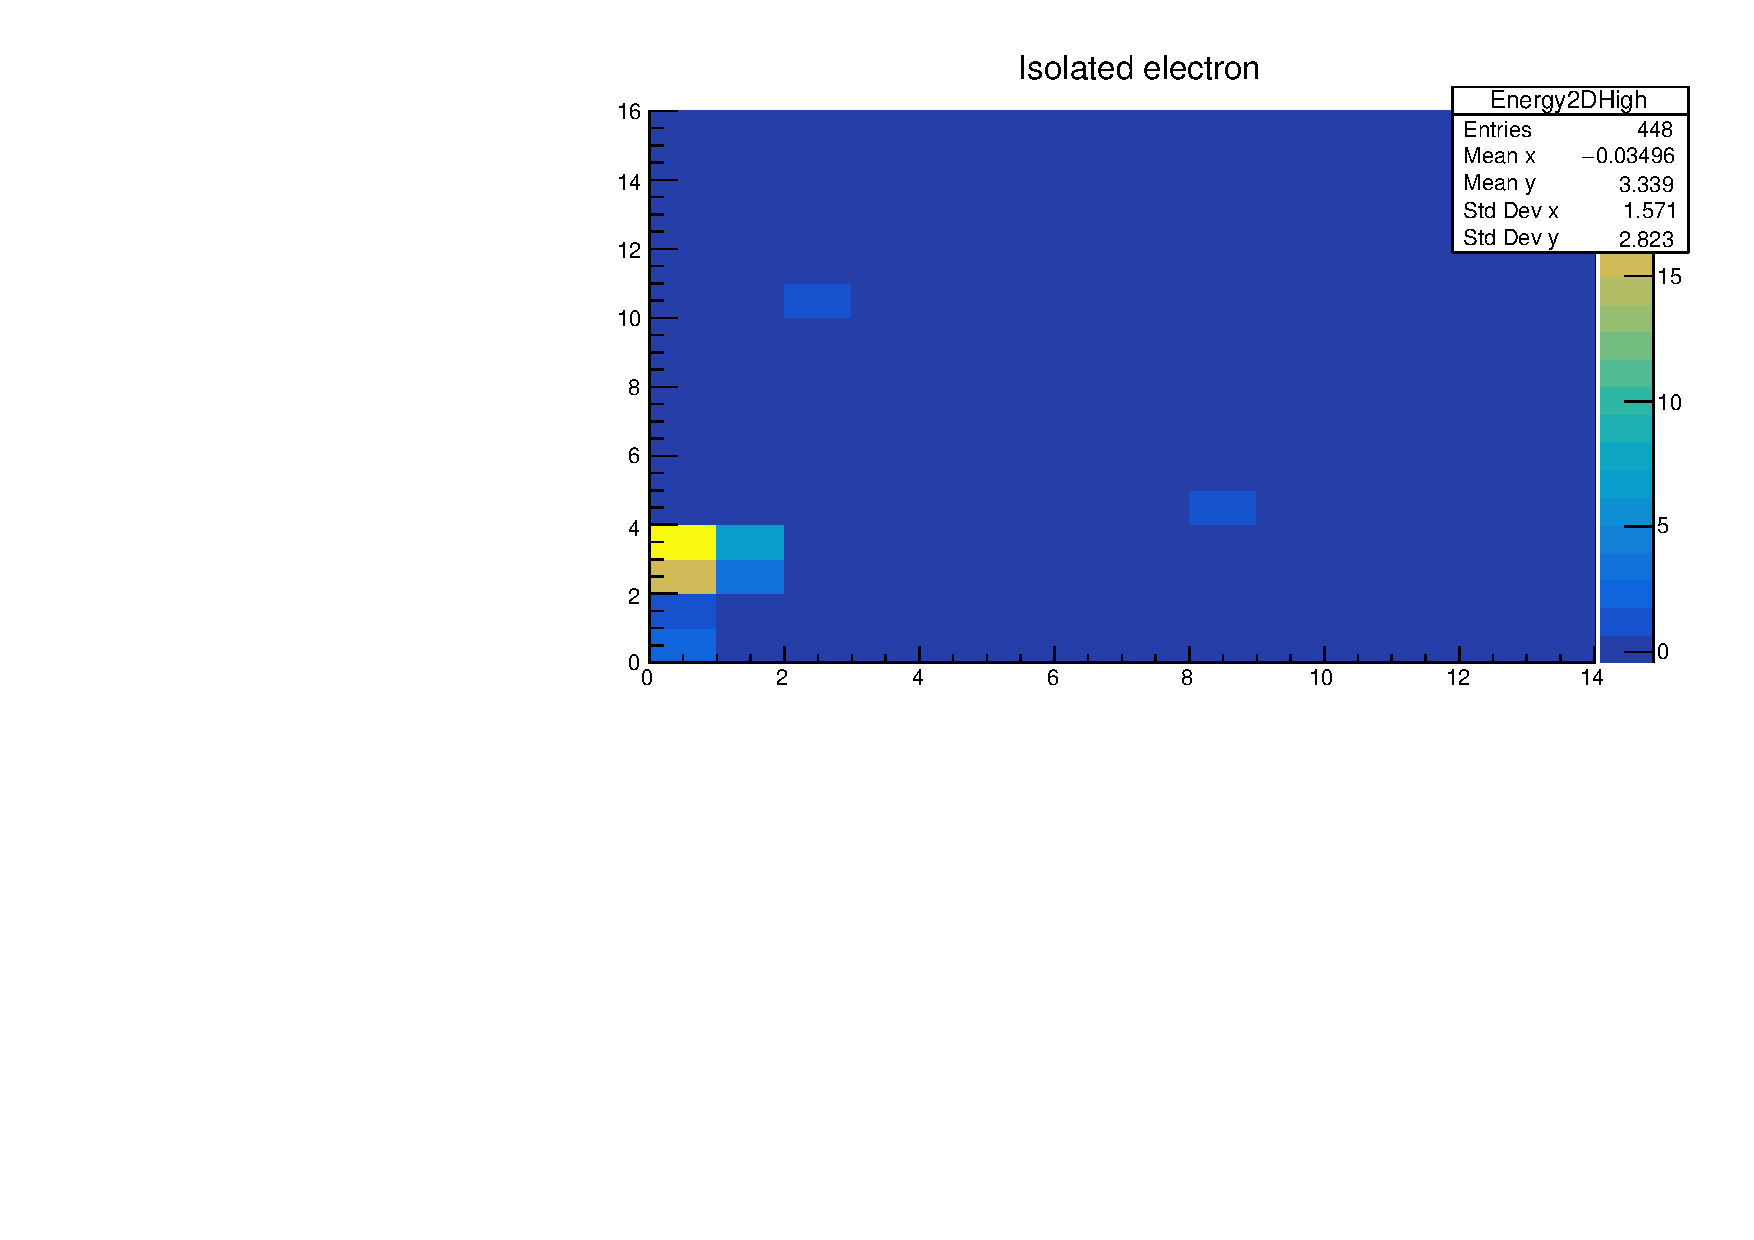
\includegraphics[width=\textwidth]{electronhist.pdf}
\end{minipage}
\begin{minipage}{0.45\textwidth}
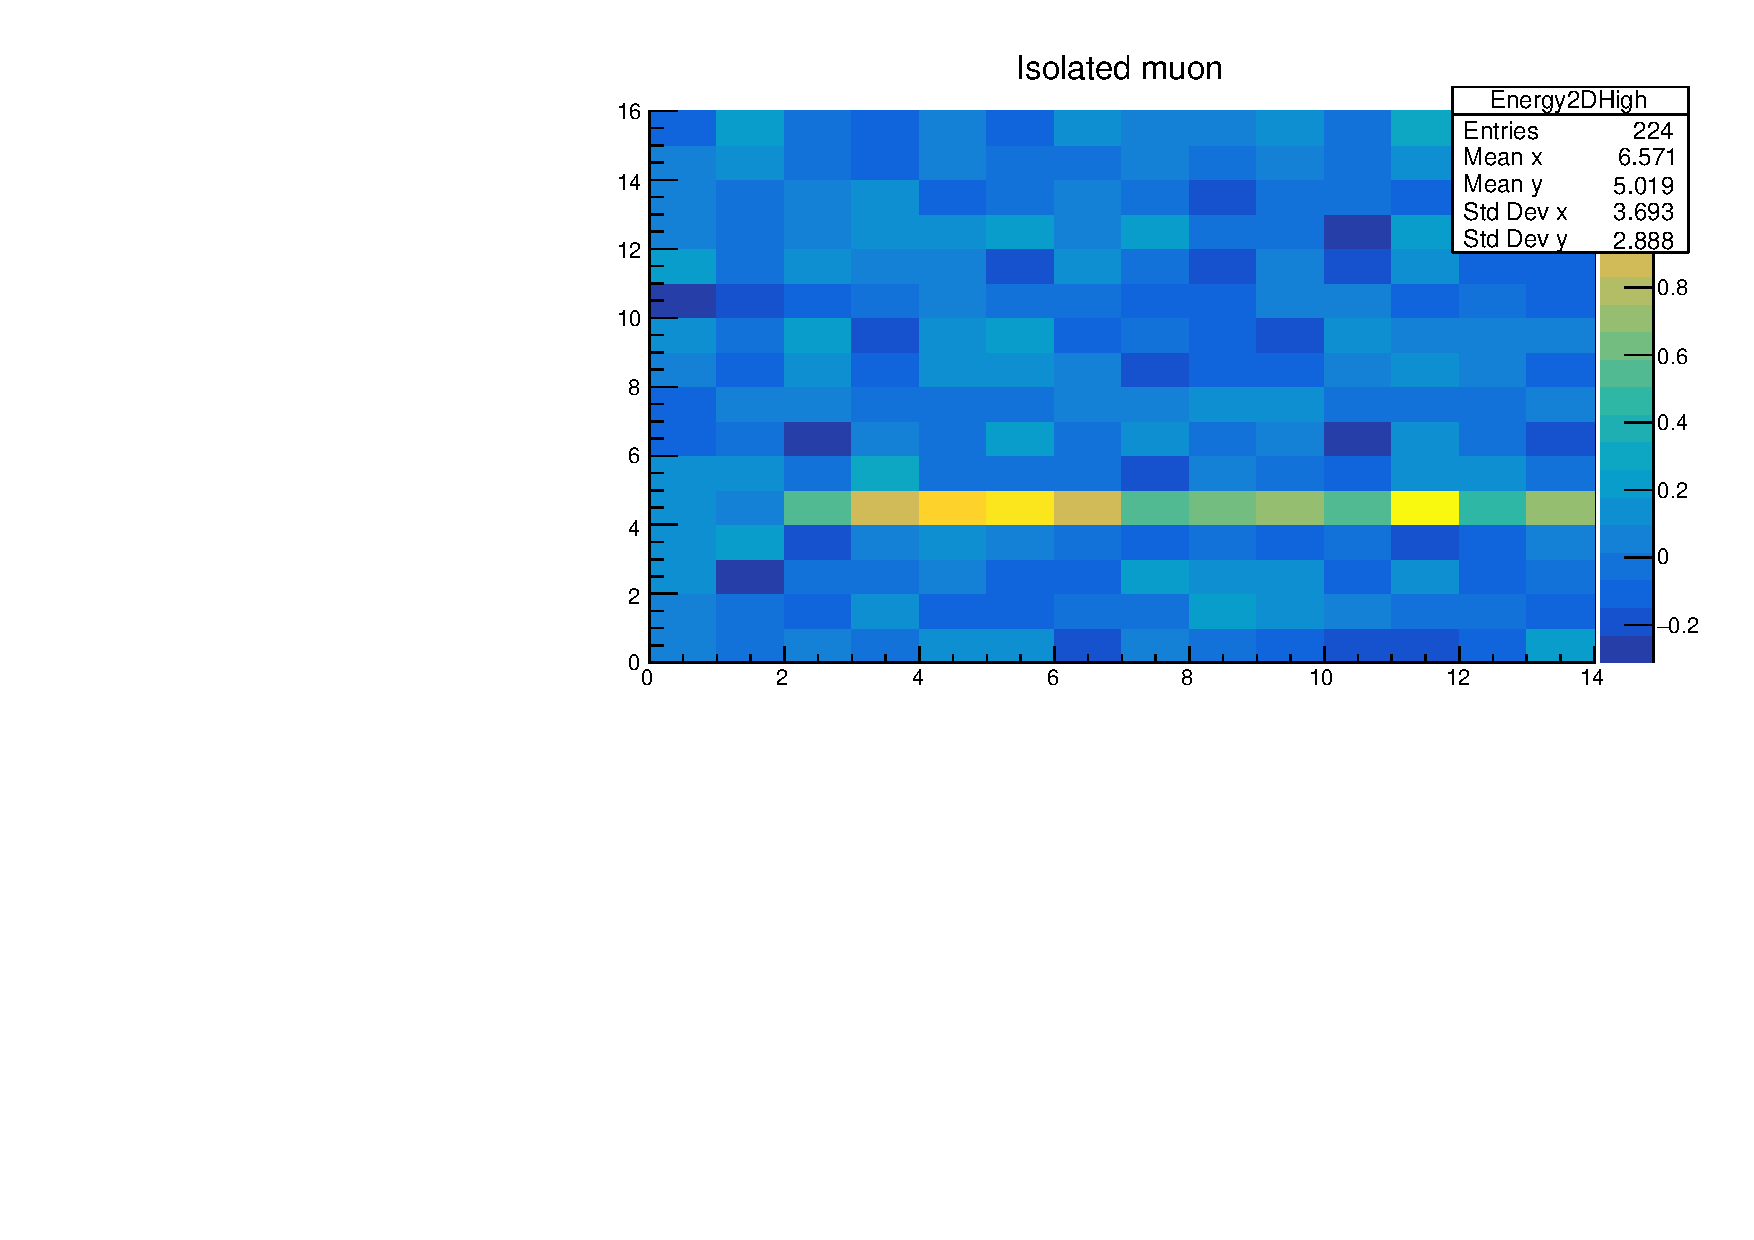
\includegraphics[width=\textwidth]{muonhist.pdf}
\end{minipage}
\end{minipage}
\begin{minipage}[b]{0.95\textwidth}
\begin{minipage}{0.45\textwidth}
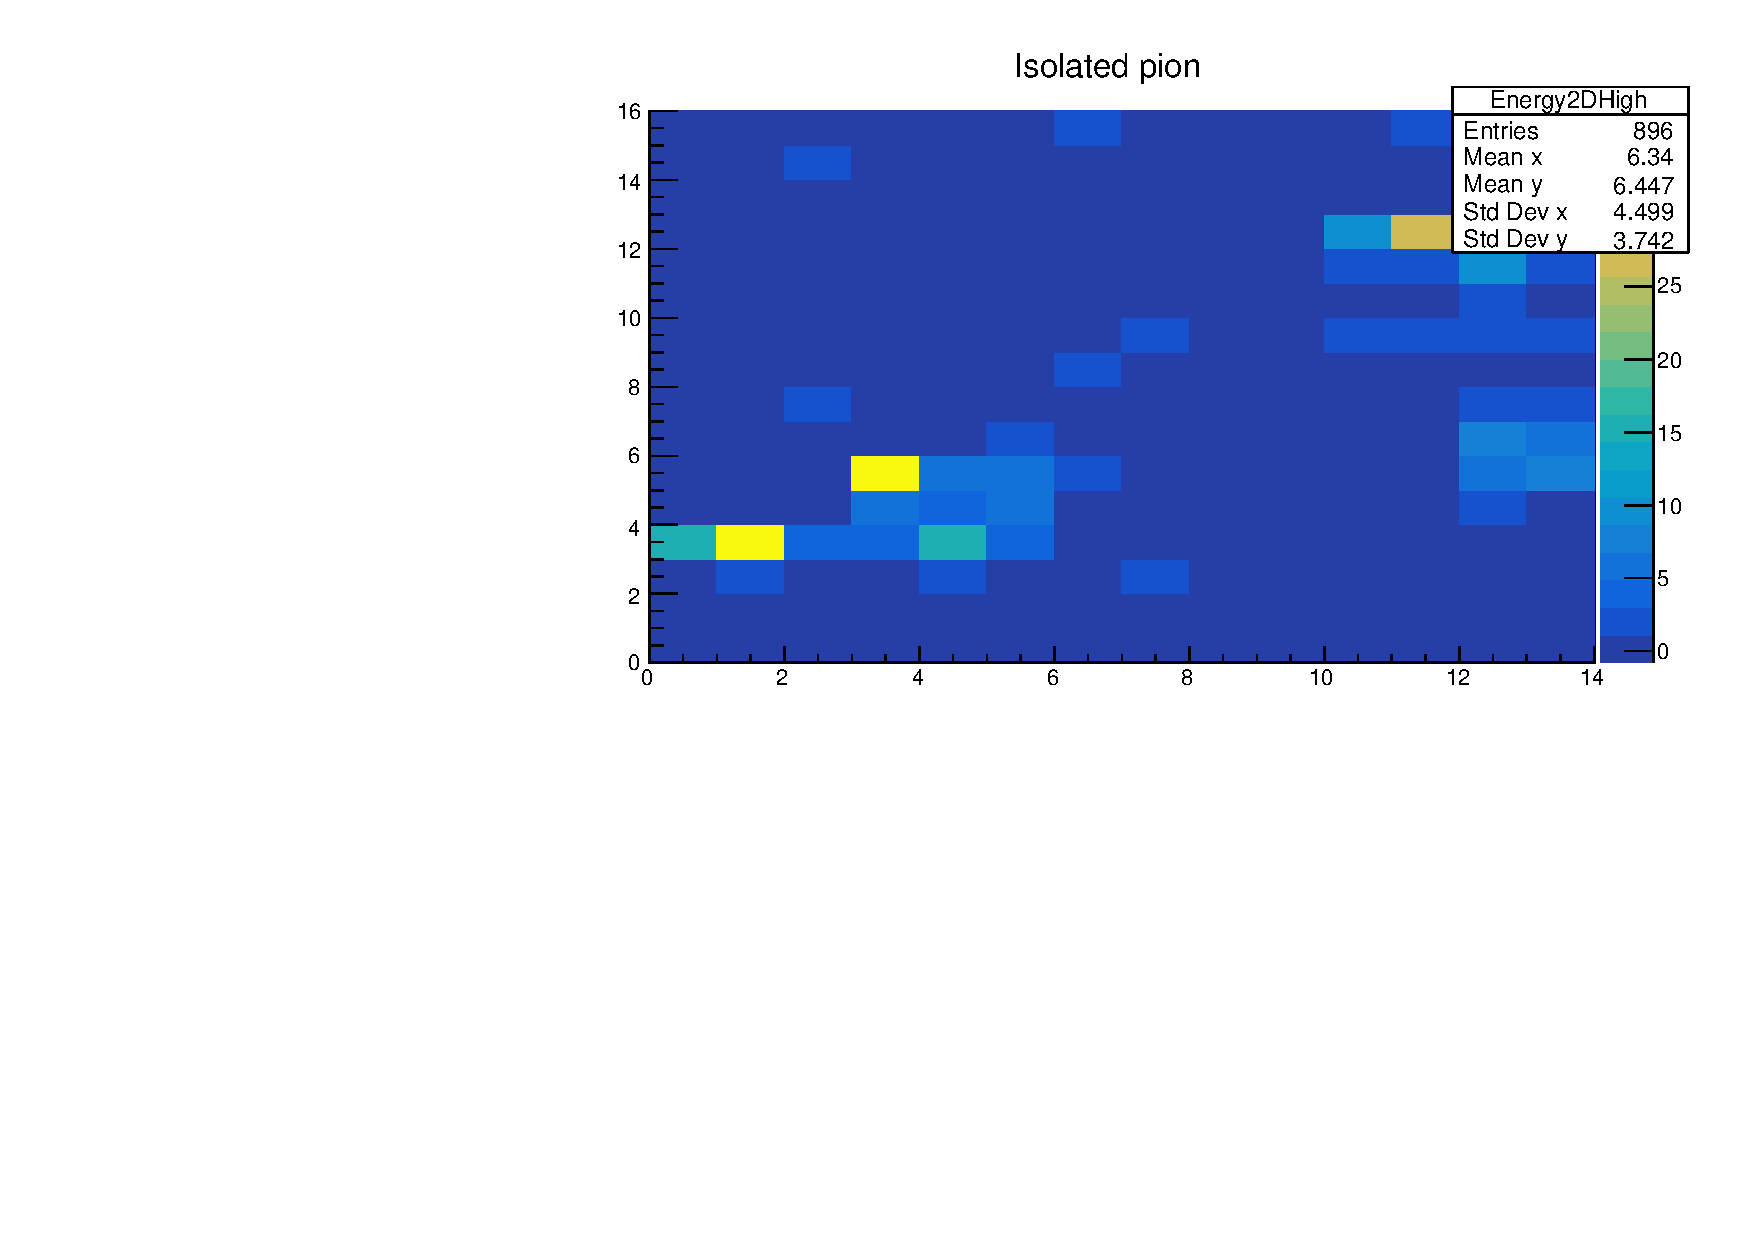
\includegraphics[width=\textwidth]{pionhist.pdf}
\end{minipage}
\begin{minipage}{0.45\textwidth}
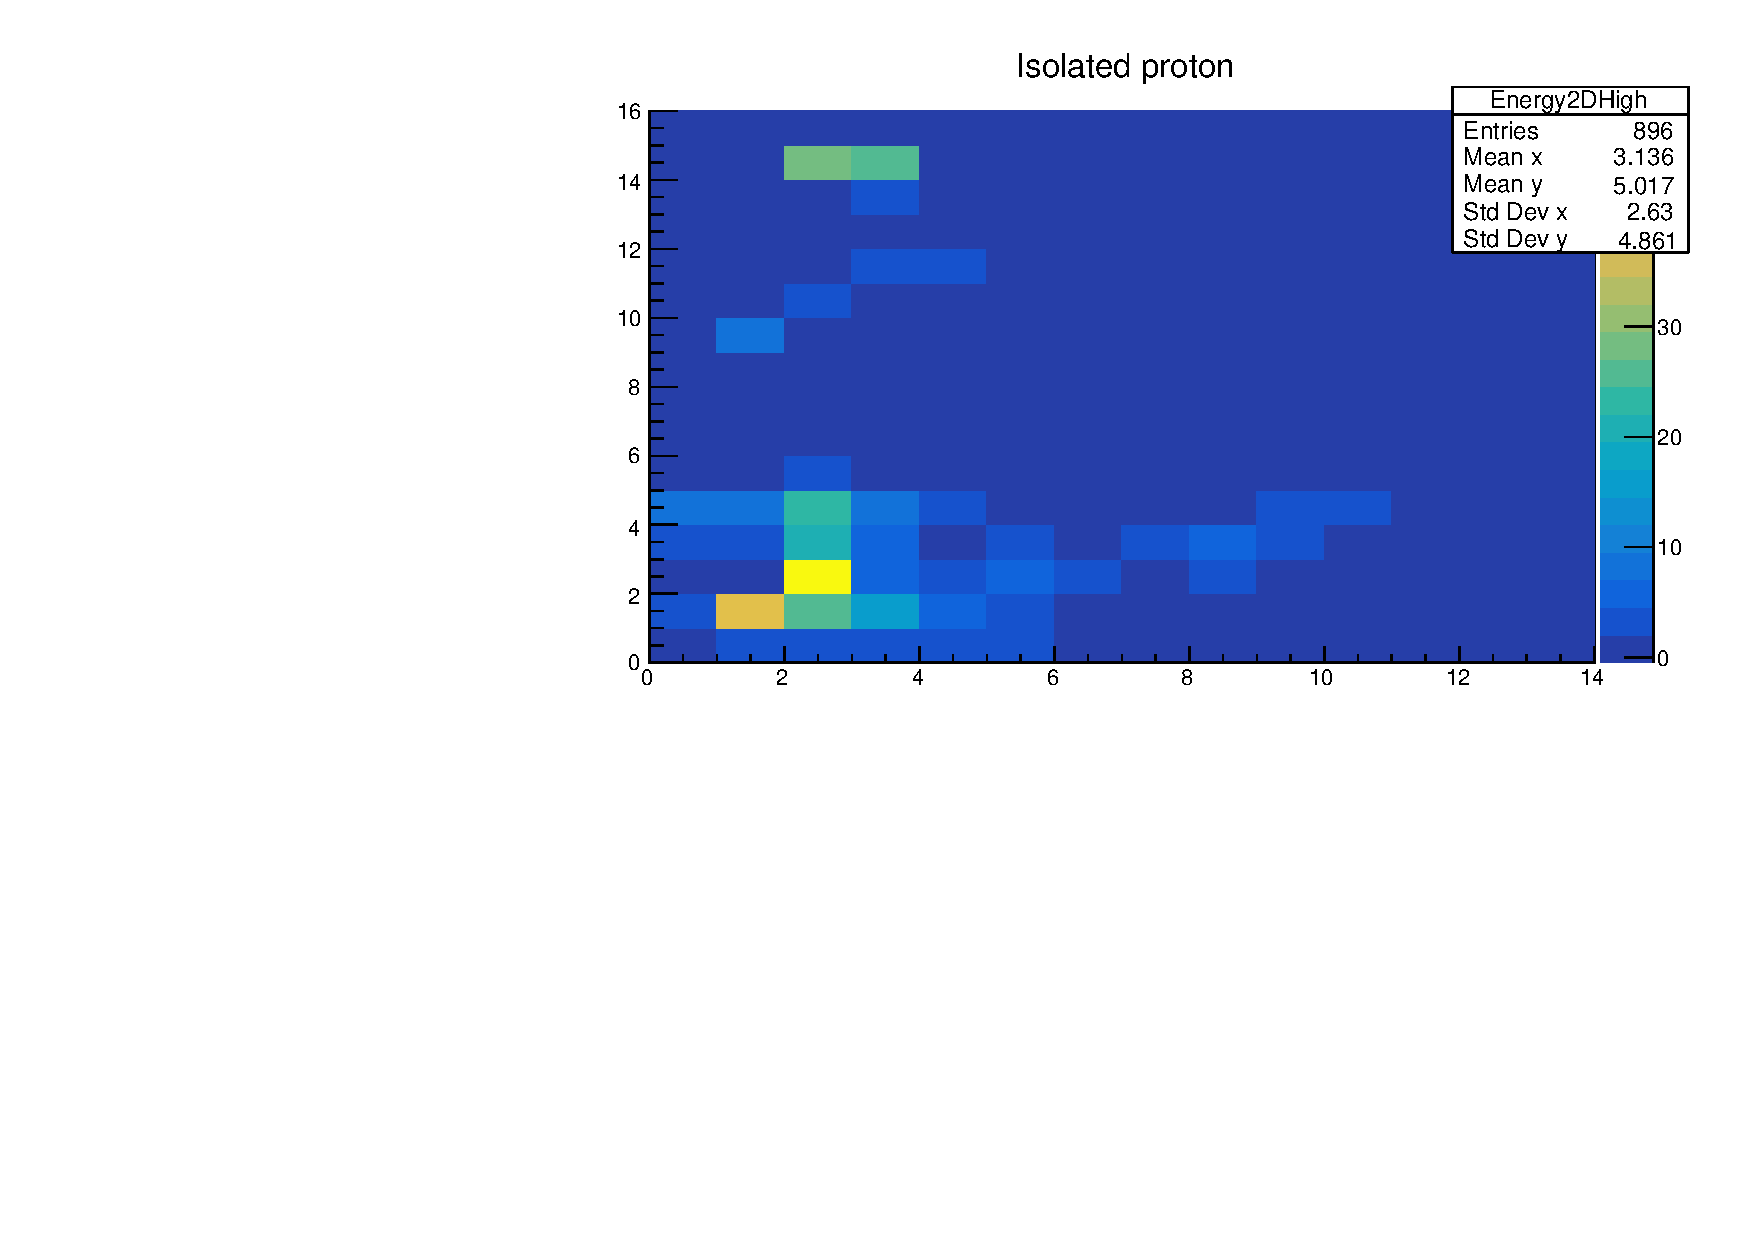
\includegraphics[width=\textwidth]{protonhist.pdf}
\end{minipage}
\end{minipage}
\caption{Energy deposit of single particles travelling through CASTOR. An electron or photon (upper left) deposits its whole energy in the electromagnetic sections, while a muon travels with only a little energy loss through every section (upper right). The signals of pions and protons is spread wider and reaches into the hadronic sections of the calorimeter (lower left and right). The data is generated by EPOS.}
\label{signals}
\end{figure}

As seen in fig. \ref{signals}, the energy deposited in CASTOR by different particles varies much. In different events particles with very different energies are created. For example the kinetic energy of a proton can be between one and several thousand GeV. To learn that these very different signals are generated by the same particle type would pose a challenge for the neural network. Every histogram is therefore normalized to 1 in signal amplitude. 
\begin{table}
\centering
\caption{Number of isolated particles travelling through CASTOR in 500.000 Monte Carlo-generated events of proton-proton collisions at $\sqrt{\mathrm{s}} = 13\,$TeV. If not specified otherwise, the numbers include the particle and the antiparticle. As can be seen, hadrons and electrons/photons dominate the spectrum.}
\sffamily
\begin{tabular}{cc |cc }
\hline
Leptons/Bosons & Count & Hadrons & Count \\ \hline
Photon & 170047 & $\pi^+$ & 106904 \\
Positron & 243 & $\pi^-$ & 103648 \\
Electron & 250 & $K^+ / K^-$ & 27591 \\
Muon & 29 & Proton & 15782\\
$\nu_{\mu}$ & 27 & Neutron & 15232 \\
$\nu_e$ & 11 & $K^0_L$ & 13604 \\
$\nu_{\tau}$ & 1 &  $\Lambda$ & 5308\\
& & $\Sigma^+$ & 2016 \\
& & $\Sigma$ & 1993 \\
& & $\Sigma^-$ & 1993 \\
& & $K^0_s$ & 1323 \\
& & $\Xi^0$ & 511 \\
& & $\Xi^-$ & 471 \\
& & $\Omega^-$ & 16 \\
 \hline
\end{tabular}
\label{particlecounts}
\end{table}
\section{Network design}
The energy deposit histograms of CASTOR can be treated as pictures with 16 to 14 pixels and varying amounts of colour intensity. In order to remove the enourmous energy dependence of the calorimeter response, all events are scaled to the same signal amplitude. To design a neural network which can classify events into particle categories techniques in image recognition should be used. In normal classification problems convolutional layers with a small and quadratic kernel size are used. Here the information given by the underlying physics can be used to the advantage of the network. 

As particles reach the calorimeter from the left, it is not useful to use small kernel sizes to cover the whole image. Small, light particles are normally contained in one tower or at most two. Therefore convolutional layers with kernel sizes of one or two towers, meaning one or two pixels in the height and 7 or 14 in the width, should be able to recognize the important features of the tracks. Several layers, each with kernel sizes with a width of 14 pixels but varying heights are concatenated in the beginning of the network. In the deeper layers of the network, smaller kernel sizes can be used, since the convolution shrinks the signal size travelling through the neurons. In fig. \ref{convnet} the network structure is shown. Because of the large kernel sizes in the beginning, the size of the data volume shrinks quickly. Max pooling was therefore omitted as too much information was lost due to the rather small input size. Deeper networks with more hidden layers have been tested but showed no advantage in accuracy. Deeper networks only need more computing time and have a higher tendency to overfit as more free parameters are available. 

\begin{figure}
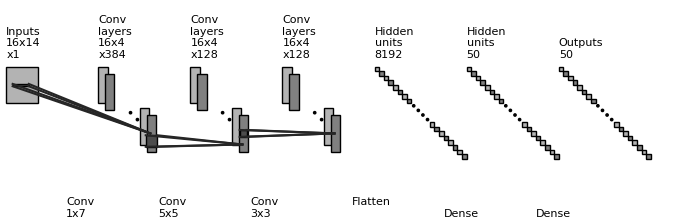
\includegraphics[scale=0.85]{convnet_fig.png}
\caption{The network design for the convolutional neural network. The first convolutional layer is composed out of kernel sizes of (1, 7), (2, 7) and (3, 7). This was omitted for a clearer picture. To reduce overfitting, dropout is used between after the first convolutional layer and before and after the first dense layer, each with a probability of 0.5. \protect \footnotemark}
\label{convnet}
\end{figure}

\section{Monitoring}
For monitoring the progress of a neural network, the first important feature is the loss function. As the classification problem is a multi-label classification, the loss function used here is the binary crossentropy loss. Every epoch it is calculated for the training and for the validation data set. Both variables need to decrease during the training. To determine if the input is correctly put into the network the first step was to train without any dropout or pooling layers. The network should overfit on the training set if given enough time. In fig. \ref{overfitacc} the loss and the accuracy of the training while overfitting can be seen.
\footnotetext{This figure is generated by adapting the code from \url{https://github.com/gwding/draw_convnet}}
\begin{figure}
\centering
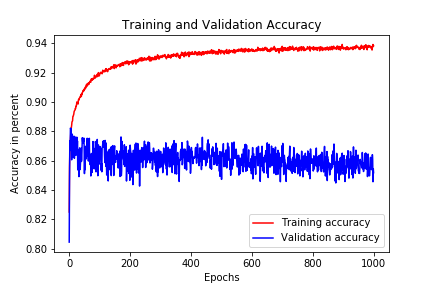
\includegraphics[scale=0.8]{trainvalacc.png}
\caption{Training and validation accuracy. Both start at roughly the same percentage, but as training goes on, the training accuracy increases constantly. The validation accuracy does not change or even decreases a little. This is a classic overfitting effect.}
\label{overfitacc}
\end{figure}
As standard networks normally deal with multi-class and not multi-label problems, it proved to be useful to additionally monitor variables commonly used in classification problems. Here recall and precision were implemented \cite{rijsbergen}. With recall, the false negatives are taken into account, while precision monitors the false positives. Recall is also called the sensitivity of a network and is calculated by
\begin{equation}
\mathrm{Recall} = \frac{tp}{tp + fn} \quad ,
\label{recall}
\end{equation}
where tp stands for true positive, tn for false negative. The recall therefore is the fraction of true positive labels over all actually positive labels. In the case of all labels being correctly predicted, the recall is 1. Precision is also referred to as the positive predictive value. It is the rate of all correctly classified positive labels over all positively predicted labels.
\begin{equation}
\mathrm{Precision} = \frac{tp}{tp + fp}
\end{equation}
The nomenclature is the same, tp for true positives and fp for false positives. When all labels are correctly predicted, the precision also equals 1.

The precision and the recall can be calculated separately for the different categories. It can be easily monitored if the networks has more problems recognizing one category over the others. 

%Another number which was monitored was the number of falsely labelled electrons. It was obvious after a few training sessions that the network had most problems classifying electrons. A counter of the falsely labelled electrons was therefore implemented in the callbacks. With y$_{\mathrm{true}}$ as the true labels and y$_{\mathrm{pred}}$ as the predicted labels, the counter worked as seen below.
%\begin{equation}
%\mathrm{count} = (1 - y_{\mathrm{true}}) \cdot y_{\mathrm{pred}} - (1 - y_{\mathrm{pred}}) \cdot y_{\mathrm{true}}
%\end{equation}
%It is the same as the crossentropy loss without the logarithm, but with two main differences. The first one is that here not the predicted probabilities are used as input put the absolute prediction. That means if y$_{\mathrm{pred}}$ is higher than 0.5 it is rounded to 1, lower than 0.5 means being rounded to 0. The second one is it being a difference rather than a sum. This way if the number is negative, the network has more false negatives than false positives, if it is positive, more false positives than negatives. 
\section{Evaluation}
In the process of training it became apparent that no real physical features were being learned by the network. The training loss decreased but the validation remained constant over several hundred epochs (fig. \ref{trainvalloss}). As mentioned before, without  regulations the network overfitted on the training data without problem. This lead to reevaluating the input data, as it seemed to be difficult for the network to generalize the underlying physical laws. 

\begin{figure}
\centering
\begin{minipage}{0.45\textwidth}
\centering
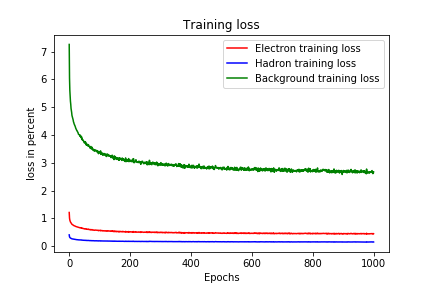
\includegraphics[scale=0.45]{trainloss.png}
\end{minipage}
\begin{minipage}{0.45\textwidth}
\centering
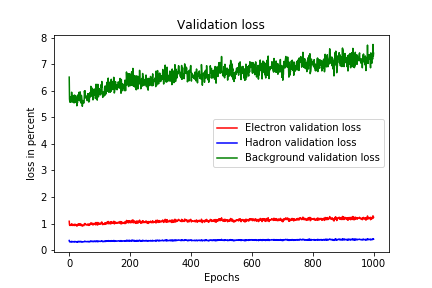
\includegraphics[scale=0.45]{valloss.png}
\end{minipage}
\caption{Training and validation loss for single particles. The training loss behaves exactly as it is supposed to, decreasing gradually during training. The validation loss shows that the network is not generalizing properly. It is remaining constant or even increasing, showing that the error rates get higher.}
\label{trainvalloss}
\end{figure}

One problem was the definition of background events. Since at first only isolated particles were considered, background events could also contain hadrons or electrons and photons, just not in the right distance to other particles travelling through CASTOR. The background category therefore contained input data which were not distinguishable from an photon or hadron event. To solve this problem, two different approaches were chosen. The first one was to completely ignore the background category and turn the classification into a binary problem, only distinguishing between electromagnetic particles, photons and electrons, and hadrons. The second was the redefinition of the background category, where only true background was used. True background meant, that no particle with an energy higher than 3 GeV had travelled through CASTOR in the corresponding signal. To further simplify the classification, only single particles were used, meaning that one particle per event crossed CASTOR. In tab. \ref{singleparticles} are the particles belonging to this data set. The background category consists mostly of no particles, which is not shown here. As single particles are rarer than isolated particles, two million events were evaluated. Still the number of useful histograms is smaller than with isolated particles, where 500.000 events were used.

\begin{table}
\centering
\caption{Single particles crossing through CASTOR. The particles in the background category are no single particles but have an energy less than 3 GeV. Two million events were evaluated.}
\sffamily
\begin{tabular}{cccc}\hline
Particle & Electromagnetic Class & Hadronic Class & Background Class \\ \hline
$\Lambda$ & 0 & 641 & 0 \\
Proton & 0 & 1915 & 0 \\
Neutron & 0 & 2355 & 0 \\
Electron  & 64 & 0 & 11 \\
Photon & 18327 & 0 & 80 \\
Pi$^{+-}$ & 0 & 25292 & 3 \\ 
K$^{+-}$ & 0 & 3608 & 0 \\
K$_l$ & 0 & 1769 & 0 \\
K$_s$ & 0 & 1812 & 0 \\
$\Omega^-$ & 0 & 3 & 0 \\
$\Xi^0$ & 0 & 53 & 0 \\
$\Xi^-$ & 0 & 52 & 0 \\
$\Sigma^+$ & 0 & 263 & 0 \\
$\Sigma^-$ & 0 & 384 & 0 \\
\hline
\end{tabular}
\label{singleparticles}
\end{table}


As precision and recall were implemented as callbacks, their value was returned after every epoch. In the first few training sessions the monitoring of these showed that while the mean loss decreased and the accuracy increased, the recall especially of electrons remained really low. To counteract this, the binary crossentropy loss was defined as a separate function. The crossentropy is the sum of two parts, one evaluating and penalizing the number of false positives, the other watching the number of false negatives. As recall, as seen in eq. \enquote{\ref{recall}}, evaluates the false negatives, they were stronger penalized than the false positives.

\subsection{Comparison between different data inputs}

To evaluate the possible applications and limits of the event classification with the help of a neural network, several data sets have been used and compared. As the first idea was to classify isolated particles, one dataset is composed of isolated electromagnetic particles, isolated hadronic particles and background, in which no isolated particle crosses CASTOR. All particles included in this data can be seen in table \ref{particlecounts}. As the background definition for this data type was difficult and the distinguishing between events with more than one particle to those with only one also seemed to worsen the performance of the network, single particles were introduced. Only events in which just one particle had crossed through CASTOR were counted here. To also better define the background class, events with particles no higher than 3 GeV or no particle in CASTOR	were included in this class. At last, a binary classification was tried, excluding the background completely. For every data type, the training and the validation loss function can be seen in fig. \ref{lossall}. The expected result would be that the network performs worse on isolated particles since the distinction between background and electromagnetic/hadronic particles was not clear. Several events could also fall in both the electromagnetic and the hadronic class, which was more difficult to recognize. As can be seen in fig. no analysis behaves at it should. The training loss decreases exponentially, which is the expected behaviour. The validation loss remains constant or increases. This should not happen as dropout of 0.5 is used during all training time. Increasing dropout had no effect on the training. As the training loss functions correctly, it can be assumed that the implementation of the network is right. It seems to be unable to identify physical features which correctly classify the events. A hadronic process is more easily identified judging by the relatively small loss function. 

\begin{figure}
\centering
\begin{minipage}{0.45\textwidth}
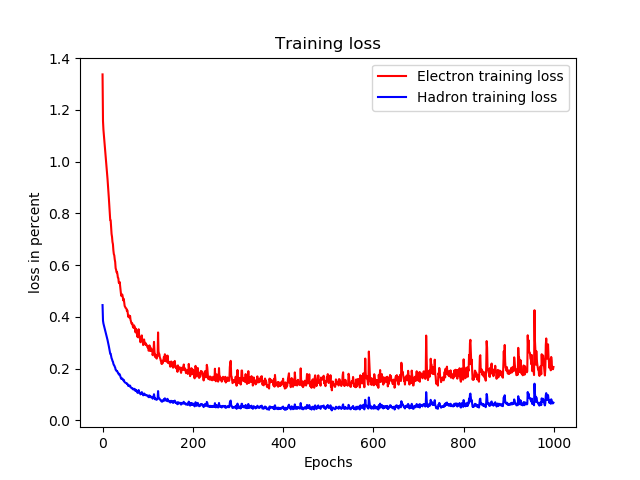
\includegraphics[width=7cm]{trainlossbinary.png}
\end{minipage}
\begin{minipage}{0.45\textwidth}
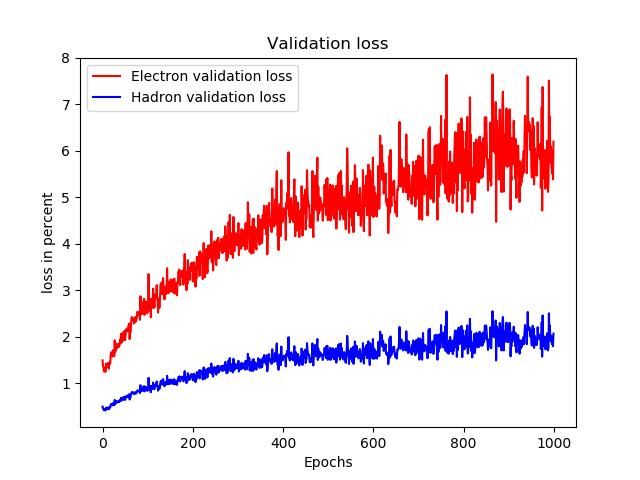
\includegraphics[width=7cm]{vallossbinary.png}
\end{minipage}
\\
\begin{minipage}{0.45\textwidth}
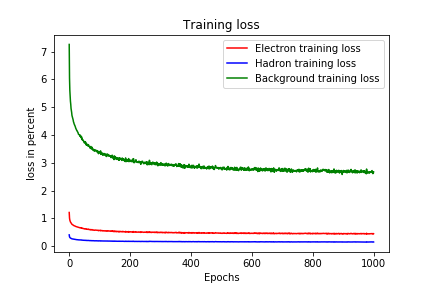
\includegraphics[width=7cm]{trainloss.png}
\end{minipage}
\begin{minipage}{0.45\textwidth}
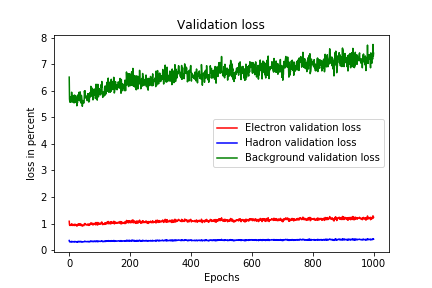
\includegraphics[width=7cm]{valloss.png}
\end{minipage}
\\\begin{minipage}{0.45\textwidth}
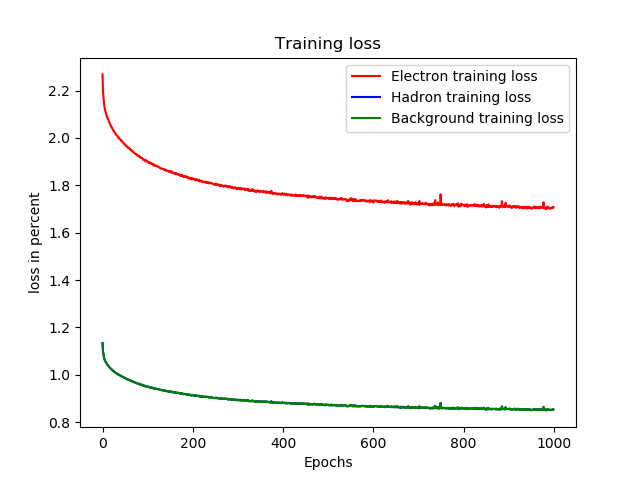
\includegraphics[width=7cm]{trainlossisolated.png}
\end{minipage}
\begin{minipage}{0.45\textwidth}
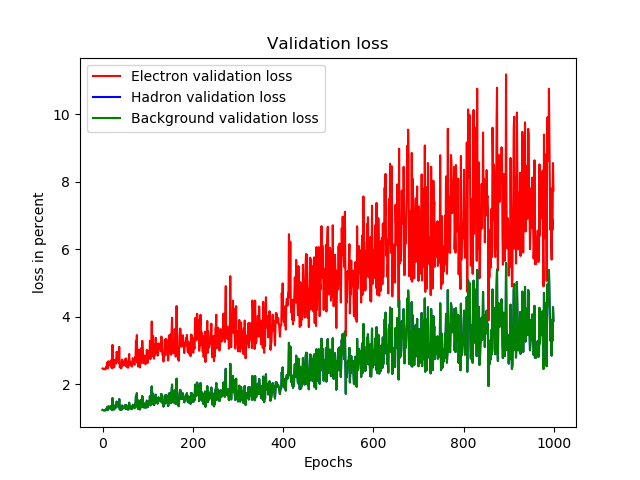
\includegraphics[width=7cm]{vallossisolated.png}
\end{minipage}
\caption{Training and validation loss for different data sets. At first the binary classification is shown, then the single particles and at last the isolated particles. The correct tendency for the loss function to decrease is seen in every training figure. The validation loss behaves not as it should. It seems to forget what it learned.}
\end{figure}

\begin{figure}
\centering
\begin{minipage}{0.45\textwidth}
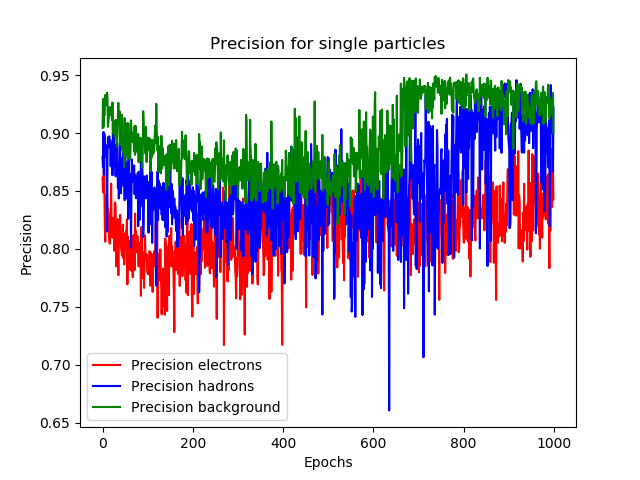
\includegraphics[width=7cm]{precisionsingle.png}
\end{minipage}
\begin{minipage}{0.45\textwidth}
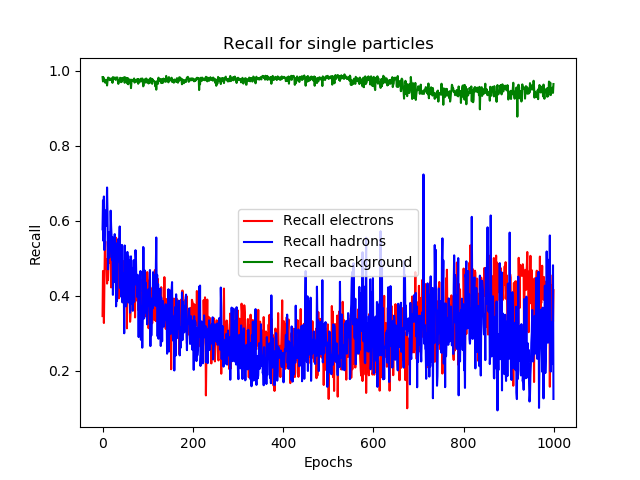
\includegraphics[width=7cm]{recallsingle.png}
\end{minipage}
\caption{Precision and recall for single particles. The precision is rather high, false positives are therefore seldom. In comparison, recall is low for electrons and hadrons. Many times the network falsely labels an event as not belonging to one of these categories but rather to the background or no class.}
\label{lossall}
\end{figure}

The single particles have the most constant performance on the validation data set but it still seems to increase during training time. The last set in fig. \ref{lossall} is the training with isolated particles. For unknown reasons the background loss function behaves exactly the same as the hadron loss function, during training as well as during validation. 
\subsection{Performance on actual data}
To see how the network performed on actual data after training, two runs with proton-proton collisions at $\sqrt{s}$ = 13 TeV with very low luminosity were evaluated. The low luminosity was useful to ensure that a high number of events contained isolated or single particles. To assess the performance of the network, the ratio of electromagnetic energy deposit contained in the first two sections of every tower to hadronic energy deposit in the following 14 sections was calculated. The energy ratio E$_{\mathrm{em}}$/(E$_{\mathrm{em}}$ + E$_{\mathrm{had}}$)is shown in the histograms in fig. \ref{ratio}, in comparison to actual electromagnetic and hadronic events and their ratio made by Monte Carlo simulations by EPOS. 
\begin{figure}
\centering
\begin{minipage}{0.45\textwidth}
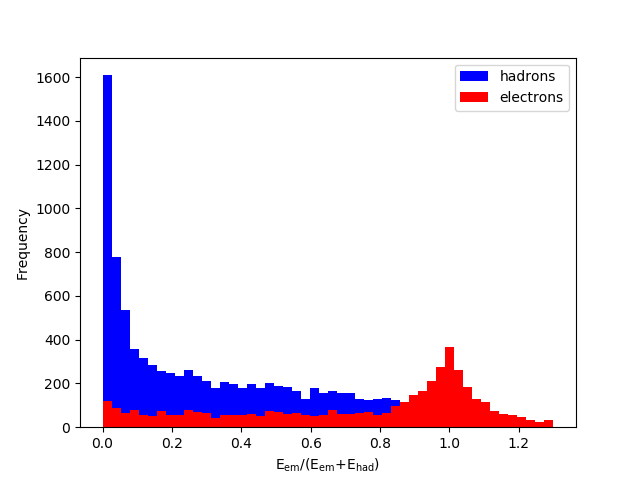
\includegraphics[width=7cm]{ratio.png}
\end{minipage}
\begin{minipage}{0.45\textwidth}
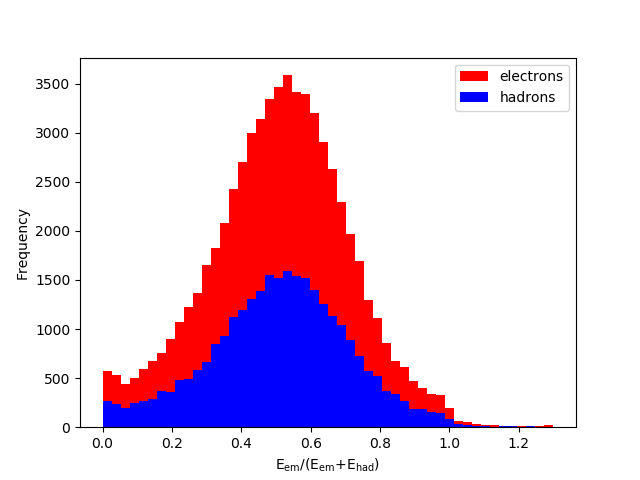
\includegraphics[width=7cm]{emhadbinary.png}
\end{minipage}
\\
\begin{minipage}{0.45\textwidth}
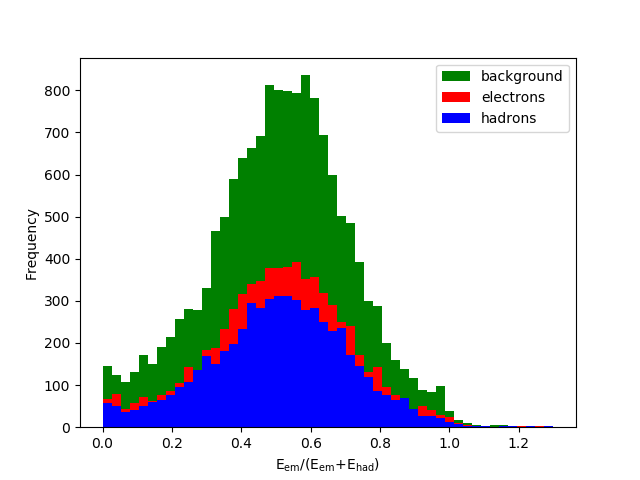
\includegraphics[width=7cm]{emhadsingle.png}
\end{minipage}
\begin{minipage}{0.45\textwidth}
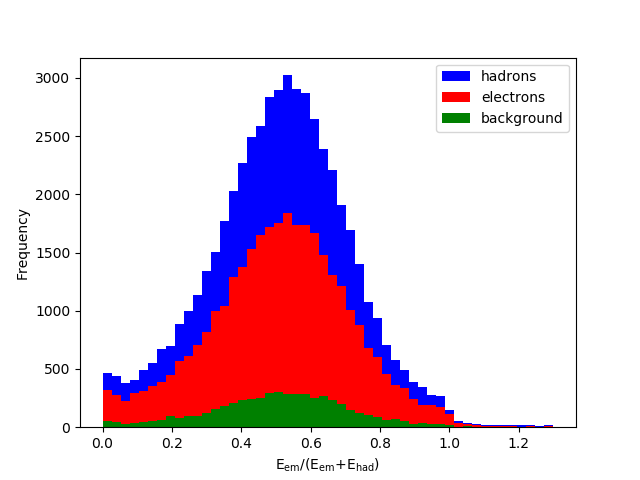
\includegraphics[width=7cm]{emhadisolated.png}
\end{minipage}
\caption{Electromagnetic to hadronic energy in the different categories. The figure on the upper left are simulated events with single electromagnetic and hadronic particles. On the upper right hand side are the ratios based on the prediction trained on binary particles. On the lower left hand side are the predictions based on single particles, on the lower right hand side the predictions based on the isolated particles.}
\label{ratio}
\end{figure}

For electromagnetic events this ratio should be nearly 1, while for hadronic events a peak at 0 is to be expected. In the simulated events this behaviourism is very obvious. There are two peaks in the histogram, one for electromagnetic and one for hadronic events. In the predicted events the tendency cannot be seen. In the real events classified by the network the energy distribution is the same for all predicted categories. As most events do not contain single or isolated particles the energy ratio is centered around 0.5. This is due to several particles per event travelling through CASTOR. Interesting is the varying amount of events predicted as CASTOR by the network trained on single and on isolated particles. As events with isolated particles can also contain several particle tracks at once more events fall into the electromagnetic or hadronic category. For single particles more events are classified as belonging to background since several particle events were excluded as training events for the other two categories.
 
The neural network is unable to correctly identify a high number of events. As in real data single or isolated particles can not be separated, many events contain several particles crossing CASTOR. This is difficult for a network to classify correctly. To see if the network is classifying at least some events accurately, events belonging to one class with a probability of at least 80 \% have been picked out. These events were then again displayed as a two dimensional histogram. An electromagnetic and a hadronic event is shown in fig. \ref{electron}. Both have been identified by the neural network trained on single particles, the networks trained on binary and isolated particles identified similar events. The signature tracks of both particle types are clearly visible. The electromagnetic particle leaves a short track, depositing its energy in the first two sections of one or two towers. A hadronic particle leaves a wider track, decaying into lighter particles, which deposit their energy throughout the detector.
\begin{figure}
\centering
\begin{minipage}{0.45\textwidth}
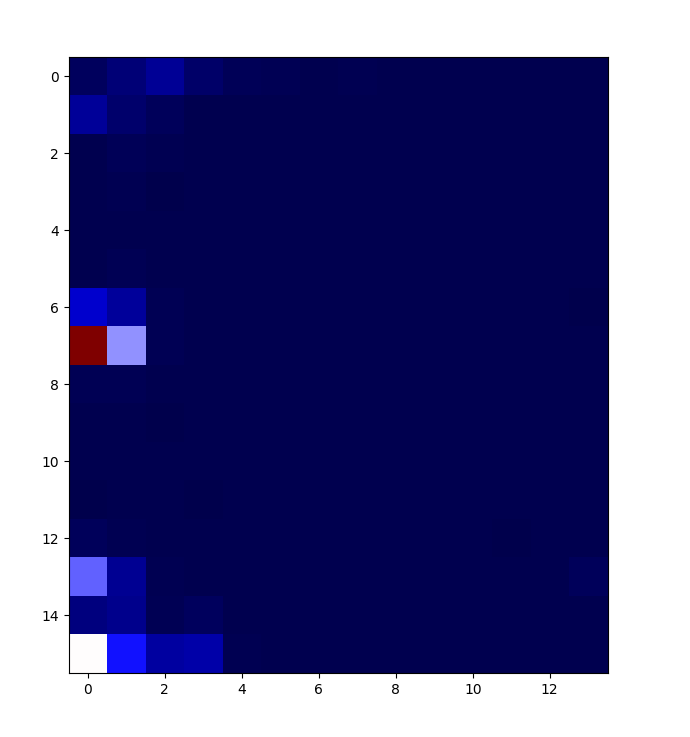
\includegraphics[width=6cm]{electron.png}
\end{minipage}
\begin{minipage}{0.45\textwidth}
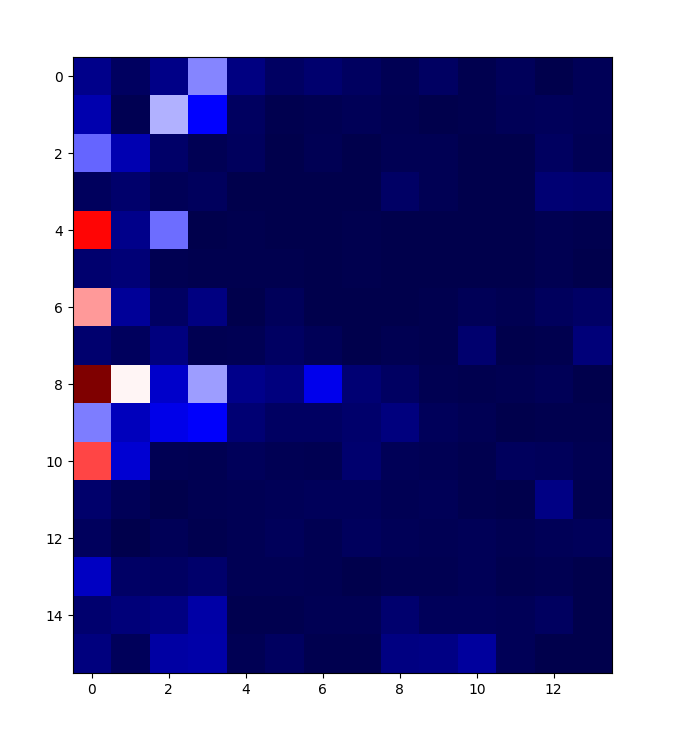
\includegraphics[width=6cm]{hadron.png}
\end{minipage}
\caption{One electromagnetic and one hadronic event with a probability higher than 80 \%. On the left the short track of an electron or photon can be seen, depositing nearly all energy in the first two sections. On the right is the wider signature of a hadron.}
\label{electron}
\end{figure}

At least a few events can be correctly identified by the neural network. The performance is not dependent on the data type used for training. Obvious particle tracks which are left by single particles can be recognized by a trained network. Overlapping signals are difficult for the network to discern and are then randomly put into one category. In real data isolated or single particles happen seldom. This explains the incorrectly behaving electromagnetic to hadronic ratio.

\subsection{Error analysis}
After several training cycles the loss function of the network still did not converge. Several possible causes for this failure have been mentioned and rectified, such as the definition of background events, very low recall and the network design. But even with only two categories, electron/photon and hadronic events, the loss function continued to show erratic behaviour. The network only performed well on very clear tracks. Events with several particles were not identified correctly. There are many possibilities which caused the poor classification, a few are going to be evaluated here.

The first one is the lack of training time. Neural networks which perform as well or even exceed human performance have an average training time of three weeks. This was not possible during this thesis as a continuous evaluation of the network's performance was needed. 

The second one is the actual distinction between hadronic and electromagnetic events with only the energy deposit as input data. As hadronic events can also cause electromagnetic showers the input signals can seem similar. If several particles cross CASTOR in one event, the overlapping signals can be difficult to distinguish. 

At last using conventional convolutional layers, important physical information gets lost. As the particles always enter the calorimeter from the left side, layers with higher weights and therefore more emphasis on the first sections could perform better than those used here. Convolutional layers share the same weights across the whole input, so no part is highlighted. This is advantageous in classic image recognition, but not for event classification in a calorimeter. 